\documentclass[
    paper = a4,
    twocolumn = true,
    %headings = normal,
    DIV = calc
]{scrartcl}

\usepackage[T1]{fontenc}
\usepackage[utf8]{inputenc}
\usepackage[english]{babel}

\usepackage{graphicx}
\usepackage[hidelinks]{hyperref}
\usepackage[numbers]{natbib}
\bibliographystyle{plainnat}

\newcommand{\mA}{mA*}
\newcommand{\GA}{GA*}


\begin{document}

\title{Final GPUC Assignment:\\
       A* GPGPU Implementations for Path-Finding}
\author{Florian Klemme}
\date{Draft -- \today}
\maketitle


\section{Introduction}

%Short description of the chosen problem. Motivations and goals of your project.

\emph{A*} is a popular search algorithm when it comes to finding the shortest path between to vertices in a graph. I will implement two different approaches of bringing the A* search algorithm to the GPU. The first approach is rather straight forward by using the parallel capabilities of the GPU to compute paths for multiple agents at the same time \cite{silva2011gpu}. In contrast, the second approach focuses on parallelizing the algorithm itself to provide maximal hardware occupancy for a single agent. \cite{zhou2015massively}


\section{Implementation}

%Discuss what parts of the problem have a parallel nature, and outline how do you plan to implement it in OpenCL. For example, which parallel programming primitives can be used.

Although both algorithms are inspired by the classic A*, their approach for parallelization is completely different. The algorithm described by \cite{silva2011gpu} (hereinafter referred to as \emph{\mA{}}) ``exploits the parallelism in performing the navigation of thousands of agents'' at the same time. The implementation should end up being quite comparable to the CPU version. The memory layout is adapted to enable coalesced memory access. A \emph{adjacency directory} is provided which allows the look-up of edges with node indices. As far as I understood this structure, depending on the graph, it might be required to have multiple copies of edges in the edge list for the look-up to work. According to the authors, the implementation of the priority queue has the biggest impact on how good this algorithm performs.

The algorithm described by \cite{zhou2015massively} (\emph{\GA{}}, as the authors call it) tries to achieve maximum parallelization for a single agent by expanding multiple nodes at a time. For this to be fast an conflict-free, \GA{} uses multiple priority queues to keep track of open nodes. New open nodes are filtered for duplicates before they are distributed back into the priority queue. Pseudocode is listed in the publication that gives a good impression on how this algorithm could be implemented. Although it might be possible to compute everything in one kernel, I think it's reasonable to split the code into one kernel for each \texttt{for ... in parallel do}. For section~\ref{sec:points}, I named those kernel by the labels from figure~\ref{fig:dataflow}. The downside of this approach is that for some information to be persistent it has to be written to global memory that -- information that otherwise could have been held in local memory. I think this only affects the priority queues and it might be able to read/write them to global memory in a coalesced manner.

\begin{figure}
    \includegraphics[page=3, trim=318 480 52 55, clip, width=\columnwidth]{zhou2015massively}
    \caption{Data flow in \GA{}. Multiple priority queues allow the conflict-free parallel extraction and expansion of multiple nodes. Syncronization is needed when it comes to cultivating the set of \emph{closed nodes}. (Image from \cite{zhou2015massively})}
    \label{fig:dataflow}
\end{figure}

For finding closed nodes, \cite{zhou2015massively} discuses different hash algorithms of which the \emph{Parallel Hashing with Replacement} algorithm is chosen for \GA{}. The pseudocode for this algorithm is not included in the article but in the separately published appendix \cite{zhou2015appendix}.


\section{Evaluation and Results}

%It is always important to specify what are the expected results of the project. For instance, when introducing an optimization of a naive algorithm, you would expect a certain amount of speed-up in advance. It is also important to examine the scalability of the application. Does the performance scale linearly with the number of computational units? If not, why? The specification is complete if it also contains ideas about evaluating the results.

Both algorithms (which means, the implementation by their authors) have already been compared to common A* CPU implementations so there are some expectations. First of all, A* on a CPU already performs quite well, so the test cases have to load the GPUs to their limits in order to shine. Both algorithms are bounded by their memory consumption so the work size will set the limit. The big difference is that \mA{} is supposed to perform well for a huge amount of agents (and consequently, a relative small graph) while \GA{} is supposed to perform well for huge graphs. Both algorithms were able to shine in their use case and I hope that I can recreate that performance in my implementation. It might be hard to compare these algorithms to one another as their strengths are so different.

In their original work, both algorithms have been evaluated using grid-like two-dimensional graphs. In \cite{silva2011gpu}, those graphs have been created automatically and paths have been chosen randomly. For \cite{zhou2015massively} the origin of test cases is not specified but by the names (``zigzag'', ``random'' and ``empty'') and a size of \(10000 \times 10000\) automatic generation is to be expected. I'll go for an automatic generation of test cases as well, as it has some advantages: Both algorithms need different test cases to show their capabilities. Specific test cases could not be reused for the other algorithm. Also for \GA{} test graphs are really big which makes it hard to find one or create one by hand. Making them two-dimensional also brings some some benefits: While developing it is easy to visualize and debug the behavior of the algorithms. At the end, nice visualizations might even be usable for the project's presentation.


\subsection{Overall points}

\begin{description}
    \item[2~points] initial concept
    \item[14~points] implementation in OpenCL
    \item[2~points] short presentation
    \item[2~points] evaluation and discussion (Q \& A)
\end{description}


\subsection{Implementation points}
\label{sec:points}

\paragraph{Priority queue} Implement priority queue (binary heap). Required for both search algorithms.
\begin{itemize}
    \item Implement \emph{push} function (1~point)
    \item Implement \emph{pop} function (1~point)
\end{itemize}

\paragraph{Multi-agent A*} as proposed by \cite{silva2011gpu}.
\begin{itemize}
    \item Set up data structures to copy required data to/from the GPU. (1~point)
    \item Implement A* kernel. One thread per agent. (2~points)
\end{itemize}

\paragraph{Parallel GA*} as proposed by \cite{zhou2015massively}.
\begin{itemize}
    \item Set up data structures to copy required data to/from the GPU. (1~point)
    \item Implement \emph{Extract \& Expand} kernel. (2~points)
    \item Implement kernel that checks if search is finished. (1~point)
    \item Implement \emph{Duplicate detection} kernel, parallel hashing with replacement \cite{zhou2015appendix}. (3~points)
    \item Implement \emph{Compute \& Push-back} kernel. (2~points)
\end{itemize}


\bibliography{Assignment}

\end{document}
